\documentclass[tikz,border=5pt]{standalone}
\usepackage{amsmath}
\usetikzlibrary{arrows.meta,positioning,calc}

\definecolor{obsfill}{HTML}{DDEBF7}
\definecolor{obsline}{HTML}{2F5597}
\definecolor{basefill}{HTML}{EFEFEF}
\definecolor{baseline}{HTML}{595959}
\definecolor{resfill}{HTML}{FBE5D6}
\definecolor{resline}{HTML}{C55A11}
\definecolor{predfill}{HTML}{E2F0D9}
\definecolor{predline}{HTML}{548235}
\definecolor{evalline}{HTML}{404040}
\definecolor{arrowgray}{HTML}{333333}

\newcommand{\mathline}[1]{%
  {\fontsize{10}{12}\selectfont\ensuremath{#1}}%
}

\begin{document}
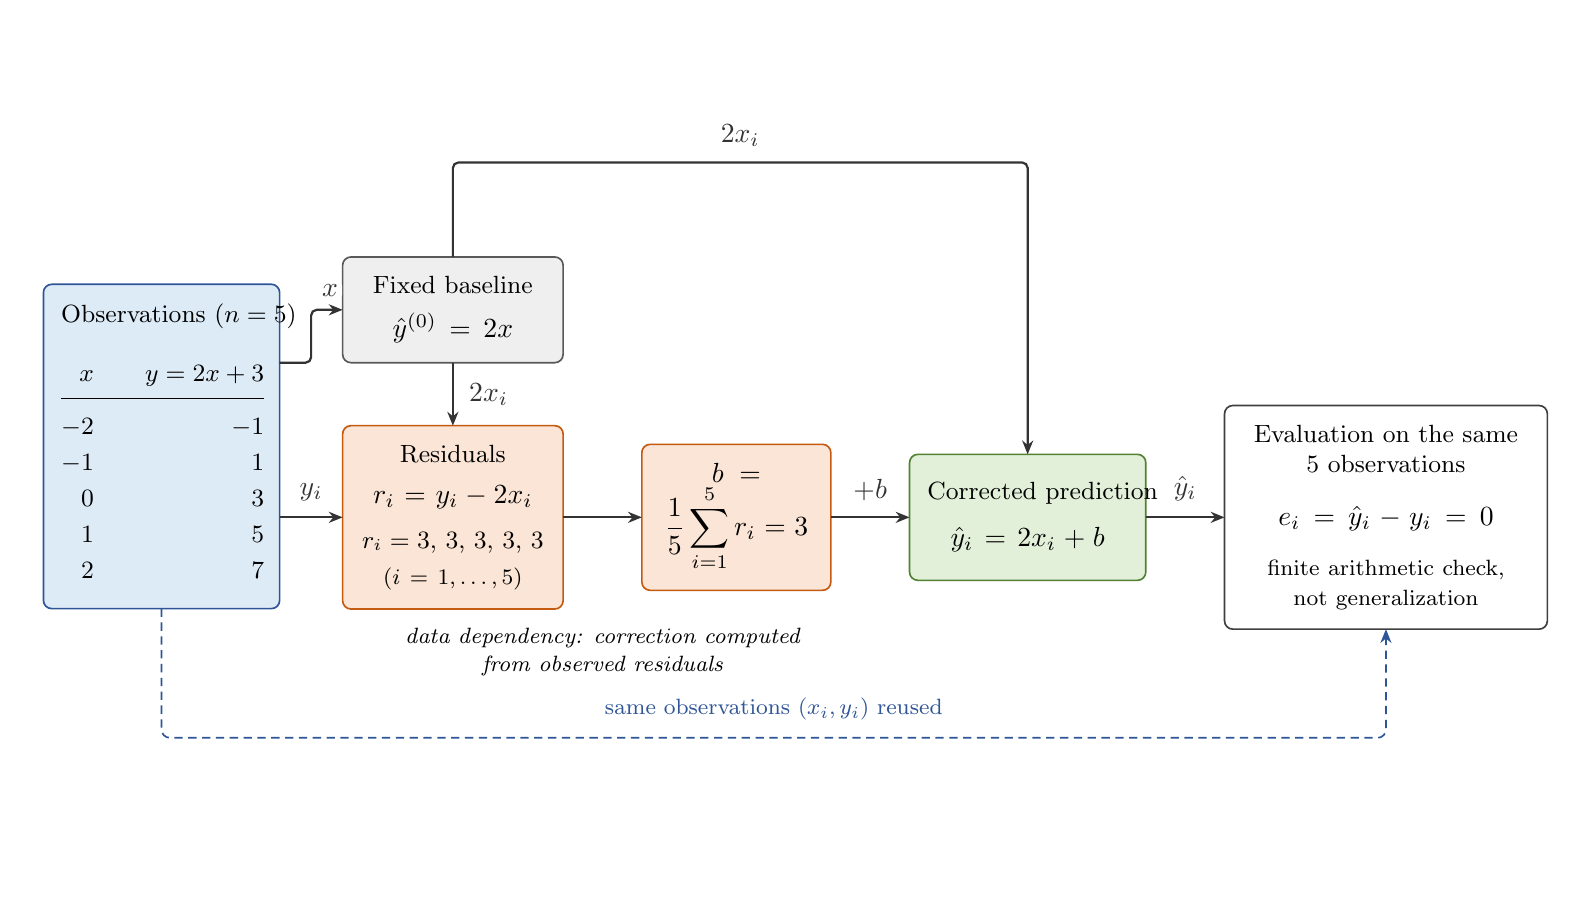
\begin{tikzpicture}[
  font=\fontsize{9}{11}\selectfont,
  box/.style={
    rectangle,
    rounded corners=3pt,
    line width=0.6pt,
    align=center,
    inner xsep=6pt,
    inner ysep=7pt,
    outer sep=0pt
  },
  observation/.style={box,fill=obsfill,draw=obsline},
  baselinebox/.style={box,fill=basefill,draw=baseline},
  residualbox/.style={box,fill=resfill,draw=resline},
  prediction/.style={box,fill=predfill,draw=predline},
  evaluation/.style={box,fill=white,draw=evalline},
  computation/.style={
    draw=arrowgray,
    line width=0.8pt,
    -{Stealth[length=5pt,width=4pt]},
    rounded corners=2pt
  },
  reuse/.style={
    draw=obsline,
    line width=0.6pt,
    dash pattern=on 3pt off 2pt,
    -{Stealth[length=5pt,width=4pt]},
    rounded corners=3pt
  },
  arrowlabel/.style={
    font=\fontsize{10}{12}\selectfont,
    fill=white,
    inner sep=1.5pt,
    text=arrowgray
  }
]

% Explicit landscape canvas: 19.5 cm by 10.96875 cm (16:9).
\path[use as bounding box]
  (-0.2,-4.55) rectangle (19.3,6.41875);
\fill[white]
  (-0.2,-4.55) rectangle (19.3,6.41875);

% Column 1.
\node[
  observation,
  minimum width=3cm,
  minimum height=3.8cm,
  text width=2.55cm
] (observations) at (1.5,1.1) {%
  \mbox{Observations ($n=5$)}\\[9pt]
  \renewcommand{\arraystretch}{1.18}%
  \begin{tabular}{@{}r@{\qquad}r@{}}
    $x$ & $y=2x+3$\\[2pt]
    \hline
    \rule{0pt}{13pt}$-2$ & $-1$\\
    $-1$ & $1$\\
    $0$  & $3$\\
    $1$  & $5$\\
    $2$  & $7$
  \end{tabular}
};

% Column 2, lower row.
\node[
  residualbox,
  minimum width=2.8cm,
  minimum height=1.8cm,
  text width=2.35cm
] (residuals) at (5.2,0.2) {%
  Residuals\\[4pt]
  \mathline{r_i=y_i-2x_i}\\[5pt]
  $r_i=3,\,3,\,3,\,3,\,3$\\[2pt]
  {\fontsize{8}{10}\selectfont $(i=1,\dots,5)$}
};

% Column 2, upper row.
\node[
  baselinebox,
  above=0.8cm of residuals,
  minimum width=2.8cm,
  minimum height=1.15cm,
  text width=2.35cm
] (fixed) {%
  Fixed baseline\\[5pt]
  \mathline{\hat{y}^{(0)}=2x}
};

% Column 3.
\node[
  residualbox,
  right=1cm of residuals,
  minimum width=2.4cm,
  minimum height=1.4cm,
  text width=1.95cm
] (correction) {%
  \mathline{\displaystyle b=\frac{1}{5}\sum_{i=1}^{5}r_i=3}
};

% Column 4.
\node[
  prediction,
  right=1cm of correction,
  minimum width=3cm,
  minimum height=1.6cm,
  text width=2.55cm
] (corrected) {%
  \mbox{Corrected prediction}\\[6pt]
  \mathline{\hat{y}_i=2x_i+b}
};

% Column 5.
\node[
  evaluation,
  right=1cm of corrected,
  minimum width=4.1cm,
  minimum height=2.3cm,
  text width=3.66cm,
  inner xsep=6pt
] (evaluation) {%
  Evaluation on the same\\
  5 observations\\[8pt]
  \mathline{e_i=\hat{y}_i-y_i=0}\\[8pt]
  {\fontsize{8}{10}\selectfont
   finite arithmetic check,\\
   not generalization}
};

% Observation-to-baseline step, kept above the observation-to-residual arrow.
\coordinate (xstart) at (observations.east |- fixed.south);
\coordinate (xstep) at ($(xstart)+(0.4,0)$);
\draw[computation]
  (xstart) -- (xstep) |- (fixed.west)
  node[pos=0.80,above=3pt,arrowlabel] {$x$};

% Observed responses and baseline predictions produce the residuals.
\draw[computation]
  (observations.east |- residuals.west)
  -- node[above=4pt,arrowlabel] {$y_i$}
  (residuals.west);

\draw[computation]
  (fixed.south)
  -- node[right=4pt,arrowlabel] {$2x_i$}
  (residuals.north);

% Residuals determine the scalar correction.
\draw[computation] (residuals.east) -- (correction.west);

\coordinate (dependency) at
  ($(residuals.east)!0.5!(correction.west)$);
\node[
  below=1.4cm of dependency,
  anchor=north,
  align=center,
  inner sep=0pt,
  font=\fontsize{8}{10}\selectfont\itshape
] {%
  \mbox{data dependency: correction computed}\\
  \mbox{from observed residuals}
};

% Baseline bypass, in its own upper corridor.
\coordinate (bypassleft) at ($(fixed.north)+(0,1.2)$);
\coordinate (bypassright) at (corrected.north |- bypassleft);
\draw[computation]
  (fixed.north)
  -- (bypassleft)
  -- node[midway,above=4pt,arrowlabel] {$2x_i$}
     (bypassright)
  -- (corrected.north);

\draw[computation]
  (correction.east)
  -- node[above=4pt,arrowlabel] {$+b$}
  (corrected.west);

\draw[computation]
  (corrected.east)
  -- node[above=4pt,arrowlabel] {$\hat{y}_i$}
  (evaluation.west);

% Reuse of the observations, below every block and annotation.
\coordinate (reuseleft) at (observations.south |- 0,-2.6);
\coordinate (reuseright) at (evaluation.south |- 0,-2.6);
\draw[reuse]
  (observations.south)
  -- (reuseleft)
  -- node[
       midway,
       above=4pt,
       fill=white,
       inner sep=2pt,
       text=obsline,
       font=\fontsize{8}{10}\selectfont
     ] {same observations $(x_i,y_i)$ reused}
     (reuseright)
  -- (evaluation.south);

\end{tikzpicture}
\end{document}